\subsection{Components}\label{sec:components}

\begin{figure}[H]
\centering
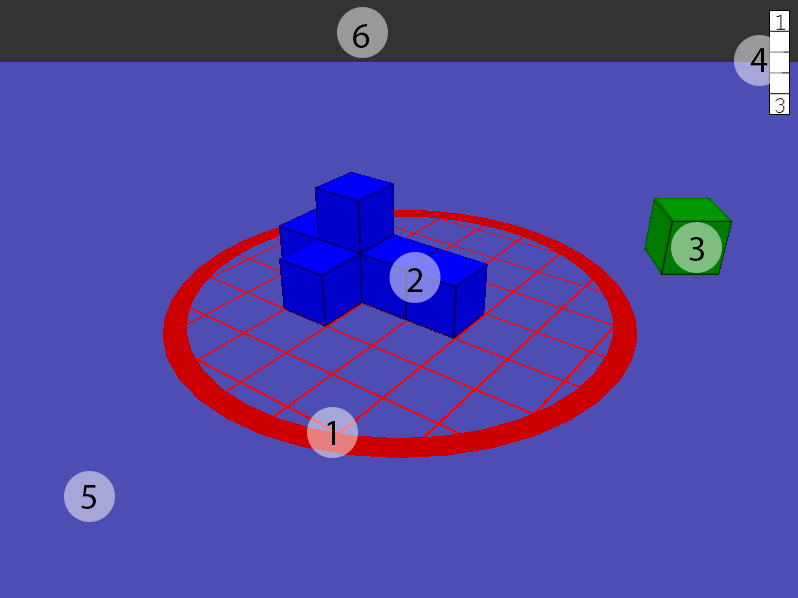
\includegraphics[width=\textwidth]{env_comps}
\caption{\label{fig:environmentcomps} Common rendering of the task environment. Visual elements: 1-Circular~grid 2-Building~blocks 3-Creation~block 4-Target~indicator 5-Floor 
6-Horizon}
\end{figure}

\noindent Figure~\ref{fig:environmentcomps} shows a common rendering of the task environment, seen through the lens of a virtual camera, in which all visual elements have been 
labeled. In the center of the screen users were presented with a circular grid that was segmented into several squares, effectively representing a grid with a circular border. 
On this grid building blocks could be positioned, either directly on the grid or stacked on top of other building blocks. New building blocks could be obtained by interacting 
(clicking with the mouse or grabbing with the Leap Motion) with the creation block just next to the circular grid. The target indicator on the top right corner gave the user a 
representation of the block structure that was supposed to be created on the grid before the user could advance.

\paragraph{Circular grid}
The circular grid was made out of square grid-cells and a limit circle with a radius that was slightly bigger than $3.5$ grid-cells width. The grid was able to rotate 
$360^{\circ}$ around the y-axis of the center of this grid (the origin). In resting state the grid and limit circle had a red color, but while the circle was rotated by the 
user the limit circle temporarily became orange until it reached resting state once more. 

\paragraph{Camera}
The camera component determined what was seen on the screen and had the origin of the circular grid as the focal point. The camera was always positioned at a fixed 
distance of $13 \frac{1}{3}$ grid-cells width from the origin of the circular grid. It started at a position in front of the circular grid under an angle of $45^{\circ}$ relative to the grid origin. The angle of the camera was modifiable in order to change the perspective on the circular grid, but the angle was limited between $1^{\circ}$ and $89^{\circ}$.

\paragraph{Building blocks}
The building blocks were 3D cubes with dimensions corresponding to $1\times 1\times 1$ the width of a grid-cell within the grid and all having black outlines at the edges. Building blocks could be lifted, dragged around, and dropped by the user. While building blocks were lifted they cast a shadow directly below them in order to let the user know their position relative to the floor and other building blocks. When building blocks were lifted and within the radius of the grid, they automatically aligned towards the grid-cells. In resting state the building blocks were blue, when they were being dragged they were orange and when a user pointed at them, but was not dragging any blocks, they became light-blue. When building blocks were released they were subjected to gravity, i.e. they fell until they hit the floor or another building block. If building blocks were released outside the circular grid they dissolved and were discarded.

\paragraph{Creation block}
The creation block was an unique fixed-position building block with the same dimensions as a building block, but with a different color. A user could use the creation block to obtain new building blocks by interacting with it. When a user pointed at the creation block it turned light-green, otherwise it had a dark-green color. In the version of the environment used for the experiment the creation block was positioned one grid-cell width above the floor level to compensate for the limited vertical detection range of the Leap Motion. Also depending on the handiness of the user the creation block was either positioned on the left (for left-handed users) or positioned on the right (for right-handed users) of the circular grid.

\paragraph{Target indicator}
The target indicator was a 2D image always visible to the user on the top right of the screen. It showed the active target goal structure that was to be created by the user during the experiment with the building blocks in order to advance to the next task and to complete the experiment. The squares corresponds to grid-cells and the numbers stated the exact amount of building blocks that were to be stacked on them. Empty squares were to contain no building blocks. The overall image thus depicted the target configuration of building blocks shown in a single orientation, but actual task completion could be achieved by creating a $90^{\circ}$, $180^{\circ}$ or $270^{\circ}$ degree rotated version of the target structure within the grid as well. Also it did not matter where in the grid the solution was created, e.g. a solution structure could be created either in the center or be translated one column to the right: both solutions would suffice. It should be noted however that for task completion the amount of building blocks required for a solution had to equal exactly the sum of all the numbers in the target model, i.e. if a solution was created with an additional building block outside the solution then the additional building block was to be removed before the user could advance. See Appendix~\ref{app:models} for the set of target models used for the experiment.


\begin{figure}[H]
\centering
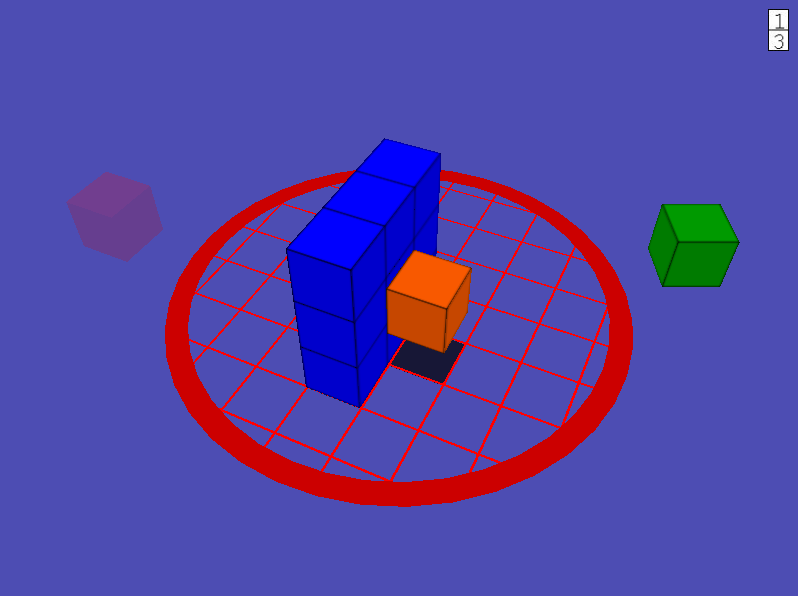
\includegraphics[width=0.47\textwidth ]{ghost_block}
\includegraphics[width=0.47\textwidth ]{Leap_hand}
\caption{\label{fig:ghostblock} \textit{On the left:} The ghost block (transparent-red block on the left) appeared when a block got stuck behind other blocks while dragging. 
In this case the user was dragging a building block from right to left, but the dragged block got stuck behind a wall of other building blocks. \textit{On the right:} The Leap 
Motion hand (transparent-green box for the palm, spheres for the finger-tops) was a visualization for when the Leap Motion device was able to detect one or more hands and the 
associated fingertips of a user. Additionally it indicated the  position of the hand palm and fingertips relative to the task environment coordinates. 
}
\end{figure}

\paragraph{Ghost block}
The ghost block was a special transparent-red block that had the same size as a normal building block. It only appeared when a building block was dragged but got stuck behind 
other blocks. Such a situation is depicted in Figure~\ref{fig:ghostblock} on the left. The ghost block helped the user to realize that an illegal dragging operation was being 
performed and what the current 3D location of the dragged building block would be if it would not have been stuck.


\paragraph{Leap Motion hand}
The Leap Motion hand visualizes the hand of the user when detected by the Leap Motion device and can be seen in Figure~\ref{fig:ghostblock} on the right. The Leap Motion 
hand was only visible to users interacting with the Leap Motion interface and helped to relate the relative position of the hands detected by the Leap Motion device to the 
coordinates of the task environment. Detected hand palms were represented as flat transparent-green boxes, where the position and orientation were determined by the position 
and orientation of the users hand palm relative to the Leap Motion device. Fingertips were represented with small transparent-green spheres and had positions relative to the
 fingertips of the user. Each individual fingertip and each hand palm was only shown when it was visible to the Leap Motion device and hidden otherwise.

\paragraph{Floor}
The floor was merely a purple-blue plane that indicates the lower limit to put the building blocks. It also served as a surface to project shadows from the building blocks on.

\paragraph{Horizon}
A small strip of horizon was made visible to help the user understand the orientation when tilting the camera up and down by changing the angle. The current color of the 
horizon was dark-gray.

\subsubsection{Color and lighting settings}

All the previously described components had one or more color states associated with them, depending on the state of the respective component and are listed in 
Table~\ref{tab:colors}. Each  color state consist out of a red (r), green (g), blue (b) and an alpha (a) component contributing to the color intensity and could 
optionally have a thin black border (outline) at the edges of the objects. Also all visual components, except the horizon, were influenced by two types of virtual lighting: 
\begin{enumerate}
	\item{\textbf{Ambient lighting:}} All color intensities were multiplied by $0.8$ on default.
	\item{\textbf{Parallel directional light:}} All the color intensities of non-transparent object surfaces perpendicular to the y-axis were restored to their original 
	color values.
\end{enumerate}


\begin{table}[H]
\centering
\begin{tabular}{|c|c|c|c|c|c|c|c|}
\hline
\textbf{object} & \textbf{state} & \textbf{r} & \textbf{g} & \textbf{b} & \textbf{a} & \textbf{outline} & \textbf{common name}\\ \hline\hline
Building block & resting & 0 & 0 & 255 & 255 & x & blue \\ 
 & dragged & 255 & 191 & 0 & 255 & x & orange \\ 
 & pointed & 138 & 149 & 255 & 255 & x & light-blue \\ \hline 
Creation block & resting & 0 & 178 & 0 & 255 & x & dark-green \\ 
 & pointed & 158 & 255 & 149 & 255 & x & light-green\\ \hline 
Ghost block & - & 255 & 0 & 0 & 51 & & transparent-red \\ \hline
Leap Motion hand & - & 0 & 255 & 0 & 77 & & transparent-green  \\ \hline 
Grid & resting & 255 & 0 & 0 & 255 & & red \\ 
 & rotating & 255 & 191 & 0 & 255 & & orange \\ \hline 
Floor & - & 77 & 77 & 179 & 255 & & purple/blue \\ \hline 
Horizon & - & 51 & 51 & 51 & 255 & & dark-gray \\ \hline 
\end{tabular}
\caption{\label{tab:colors} Color states of the objects within the task environment.}
\end{table}

\noindent The first reason for the different colors was that a user should be able to clearly differentiate between the components and their states within the environment. 
The outlines were added to the blocks blocks to enable the user to clearly distinguish between building blocks while they were immediately next to each other. Also, pilot
 tests without the `pointed' states for the creation block and the building blocks showed that some users struggled with identifying whether they were at the right position 
 with the Leap Motion hand to properly select and pickup blocks, thus the `pointed' states were included to make this more evident. 

